% =====================================================================
%  한국어 보고서 — 반드시 XeLaTeX 또는 LuaLaTeX 로 컴파일하세요.
%  Overleaf: Menu → Settings → Compiler → XeLaTeX
%  (pdfLaTeX 로는 한글이 깨집니다. ACL 템플릿도 비라틴 문자는 XeLaTeX 권장.)
% =====================================================================
\documentclass[11pt]{article}

% "review" → "final" 로 바꾸면 최종(저자명 표시) 버전이 됩니다.
\usepackage[review]{acl}

\usepackage{times}
\usepackage{latexsym}
\usepackage[T1]{fontenc}
\usepackage[utf8]{inputenc}
\usepackage{microtype}
\usepackage{inconsolata}
\usepackage{graphicx}
\usepackage{booktabs}
\usepackage{amsmath}
\usepackage{kotex}          % 한글 지원 (XeLaTeX/LuaLaTeX 필요)

\title{거대 언어 모델의 논리 표현 분리·수정(LCF) 재현 연구:\\
논리--내용 분리(disentanglement)가 발현되지 않을 때}

\author{저자 이름 \\
  소속 / 주소 1 \\
  소속 / 주소 2 \\
  \texttt{email@domain} \\}

\begin{document}
\maketitle

\begin{abstract}
본 보고서는 \citet{wu2025lcf}의 Logic Control Framework(LCF)를 재현한다. LCF는
추론 시점에 언어 모델의 은닉 표현(hidden state)을 \emph{내용(content)} 공간과
\emph{논리(logic)} 공간으로 분리하고, 논리 공간만 ``논리적으로 타당한'' 영역으로
이동시켜 내용을 해치지 않으면서 논리적 타당성을 높인다고 주장한다. 원 논문은 코드를
공개하지 않으므로 우리는 이를 백지에서 재구현하고, 합성 데이터로 핵심 모듈이 설계대로
동작함을 단위 검증하였다. 그러나 \textsc{Vicuna-7b}의 실제 은닉 표현에 적용했을 때
핵심 메커니즘이 발현되지 않았다. 대조 학습은 논리 공간에서 타당/비타당 표현을 분리하지
못했고(t-SNE 상 두 클래스가 완전히 혼재, 최근접-중심 분리도 최대 $0.66$으로 우연 수준
$0.5$에 근접), 그 결과 논문의 개선이 재현되지 않았다. 오류 식별(fallacy
identification) 정확도는 작은 조정 강도에서는 변화가 없고 논문 설정($\eta{=}4.5$)에서는
$3.3$\%p 하락했으며, 강력한 LLM 판별기로 측정한 결론 생성(conclusion generation)
타당성은 $36.2\%$에서 $31\text{--}35\%$로 떨어졌다. 두 가지 통제 실험으로 가장 유력한
원인 후보를 기각한다. 4-bit를 fp16으로 바꾸어도, 학습 라벨을 Claude로 고품질화해도
분리도는 우연 수준에 머물렀다. 우리는 이 실패가 ``동일 내용·반대 타당성 결론이 은닉
공간에서 선형 분리 가능하다''는 방법의 핵심 가정에서 비롯되며, 이 가정이 자원 제약하의
충실한 재현에서는 충족되지 않음을 논증한다.
\end{abstract}

\section{서론}
거대 언어 모델(LLM)은 대규모 정렬(alignment) 이후에도 전제로부터 따라 나오지 않는
결론, 즉 \emph{논리적 오류(logical fallacy)}를 여전히 생성한다 \citep{wu2025lcf}. 더
미묘한 문제는 LLM의 은닉 표현이 \emph{내용에 얽혀(content-entangled)} 있다는 점이다.
논리 구조가 같아도 출력의 타당성이 표면적 내용에 따라 달라지므로
\citep{dasgupta2024content}, 표현을 ``타당한'' 영역으로 단순히 밀면 내용까지 함께
교란된다.

\citet{wu2025lcf}는 뇌에 내용 독립적 추론 회로가 존재한다는 증거
\citep{monti2012logic}에 착안하여 LCF를 제안한다. LCF는 각 어텐션/MLP 출력을 내용
공간과 논리 공간으로 사영하고, 논리 표현만 조정 벡터(steering vector)로 타당 영역을 향해
이동시킨 뒤, 변경되지 않은 내용과 다시 융합한다. 논문은 6개 LLM에서 큰 개선을
보고한다(예: Vicuna 결론 타당성 $58.8\!\to\!75.0$).

본 보고서는 \emph{통제된 재현(controlled reproduction)}이다. 기여는 다음과 같다.
(i) LLM과 무관하게 단위 검증된, 공개·백지 재구현;
(ii) 두 과제 전부와 조정 강도 스윕, t-SNE 분석을 포함한 \textsc{Vicuna-7b} 종단 평가;
(iii) 방법이 \emph{왜} 재현되지 않는지를 분리해 내는 두 통제 실험(추론 정밀도, 학습 라벨
품질). 결과는 부정적이지만 유익하다. LCF가 의존하는 분리 구조가 발현되지 않으며, 그
책임이 어느 가정에 있는지를 규명한다.

\section{방법 개요 (LCF)}
LCF는 트랜스포머 각 블록의 어텐션·MLP 모듈 뒤에 삽입되는 작은
신경망이다 \citep{vaswani2017attention}. 두 MLP 사영기가 은닉 표현
$R_{\text{input}}$을 내용 표현 $R_{\text{content}}$와 논리 표현 $R_{\text{logic}}$로
매핑한다. 논리 표현만 전역 \emph{타당 방향} $\mathbb{V}$를 더해 수정하고(식
\ref{eq:steer}), 교차 어텐션 디코더가 내용과 수정된 논리를 재결합한 뒤(식
\ref{eq:fuse}) 은닉 표현을 그 결과 쪽으로 이동시킨다(식 \ref{eq:nudge}):
\begin{align}
R_{\text{logic}+} &= R_{\text{logic}} + \mathbb{V},\;\;
\mathbb{V} = C^{\text{pos}}_{\text{logic}} - C^{\text{neg}}_{\text{logic}}
\label{eq:steer}\\
R_{+} &= \mathrm{MLP}\!\left(R_{\text{content}} + \mathrm{Attn}(R_{\text{content}}, R_{\text{logic}+})\right)
\label{eq:fuse}\\
R_{\text{input}+} &= R_{\text{input}} + \tfrac{R_{+}-R_{\text{input}}}{\lVert R_{+}-R_{\text{input}}\rVert_2}\,\eta
\label{eq:nudge}
\end{align}
사영기와 디코더는 (LLM은 동결한 채) 재구성 손실 $\mathcal{L}_{\text{rec}}$, 논리 공간에
대한 대칭 지도 대조 손실 $\mathcal{L}_{\text{logic}\pm}$ \citep{wang2020understanding}
(같은 타당성 표현은 끌어당기고 반대 타당성 표현은 밀어냄), 그리고 동일 내용 쌍에서 논리
표현을 교환하면 타당성이 뒤집히도록 강제하는 내용 제약 $\mathcal{L}_{\text{content}}$로
학습된다. 추론 시에는 검증셋 \emph{변별력(distinctiveness)}이 가장 높은 10개 탭만
수정한다.

\section{구현}
논문이 코드를 공개하지 않으므로 식과 보충자료의 학습 절차로부터 재구현하였다(사영기
$d\!\to\!2048\!\to\!1024$; 교차 어텐션 디코더 $1024\!\to\!2048\!\to\!d$). 먼저 임의의
LLM과 무관하게 \emph{합성 데이터}에서 모듈을 검증하였다. 타당성을 알려진 축에 인코딩한
데이터에서 학습 후 재구성·내용 손실이 0에 수렴하고, 논리 공간이 깨끗이
분리되며(클래스 내 코사인 $\approx\!1.0$, 클래스 간 $\approx\!-0.78$), 조정이 비타당
표현을 타당 영역으로(양방향 제어에서는 그 반대로) 이동시킴을 확인하였다. 즉 메커니즘은
정확히 구현되었다.

\paragraph{데이터.} LFUD \citep{li2024lfud}를 사용한다(67 시나리오 $\times$ 12 오류
유형 $=804$ 항목). 시나리오 단위로 45/5/17 분할하여 540/60/204로 나누어 테스트셋이 미관측
시나리오만 포함하도록 하였다. 각 항목에서 전제와 오류 결론을 추출하고, 짝이 되는
\emph{타당} 결론은 생성한다(논문은 GPT-3.5-turbo + 수작업 검수).

\paragraph{추출·학습.} 각 (전제, 타당, 비타당) 삼중항에 대해 \texttt{전제+타당}과
\texttt{전제+비타당}을 모델에 통과시켜 10--30층의 어텐션/MLP 출력을 포착하고, 두 결론의
동일 토큰을 정렬하여 동일 내용·반대 타당성 표현 쌍을 기록한다(535개 항목에서 9{,}336쌍).
모든 탭으로 단일 LCF를 학습한 뒤 조정 벡터를 계산하고 변별력 상위 10개 탭을 선택한다.

\paragraph{논문과의 차이(표 \ref{tab:setup}).} 핵심 차이는 단일 베이스 모델,
\textbf{4-bit 양자화}, 로컬/API로 생성한 타당 결론, 그리고 논문의 GPT-4 판별기를 대신한
LLM 판별기이다. 또한 논문의 학습률($10^{-3}$)은 교차 어텐션 디코더에서 \emph{발산}하였고
(재구성 손실이 $80$ 이상으로 급등), 기울기 노름 클리핑을 동반한 $10^{-4}$가 안정적이어서
이를 사용한다.

\begin{table}[t]
\centering\small
\begin{tabular}{ll}
\toprule
구성 요소 & 본 재현 \\
\midrule
베이스 LLM & Vicuna-7b-v1.5 (4-bit NF4) \\
GPU & H100 1대의 $\sim$16--30\,GB 슬라이스 \\
타당 결론 출처 & Vicuna(및 Claude, \S\ref{sec:controlled}) \\
타당성 판별기 & Claude-Sonnet-4.6 \\
최적화 & AdamW, lr $10^{-4}$, grad-clip 1.0 \\
$\tau$ / 에폭 & 0.2 / 15 \\
\bottomrule
\end{tabular}
\caption{재현 설정과 주요 차이점.}
\label{tab:setup}
\end{table}

\section{실험 결과}
\paragraph{분리가 발현되지 않는다.}
LCF가 의존하는 메커니즘은 타당/비타당 추론이 분리되는 논리 공간이다. 이것이 나타나지
않는다. 그림 \ref{fig:tsne}은 검증 표본의 t-SNE이다. 타당(파랑)과 비타당(빨강)이
\emph{내용 공간과 논리 공간 모두}에서 혼재한다. 논문이 논리 공간에 뚜렷한 경계를
보고하는 것과 대조적이다. 정량적으로 탭별 최근접-중심 분리도는 최대
$\mathbf{0.66}$(우연 $=0.5$)이고, 대조 손실은 학습 내내 거의 평평하다. 사영기가 동일
토큰의 내용으로부터 논리적 타당성을 분리하는 방향을 끝내 찾지 못함을 의미한다.

\begin{figure}[t]
\centering
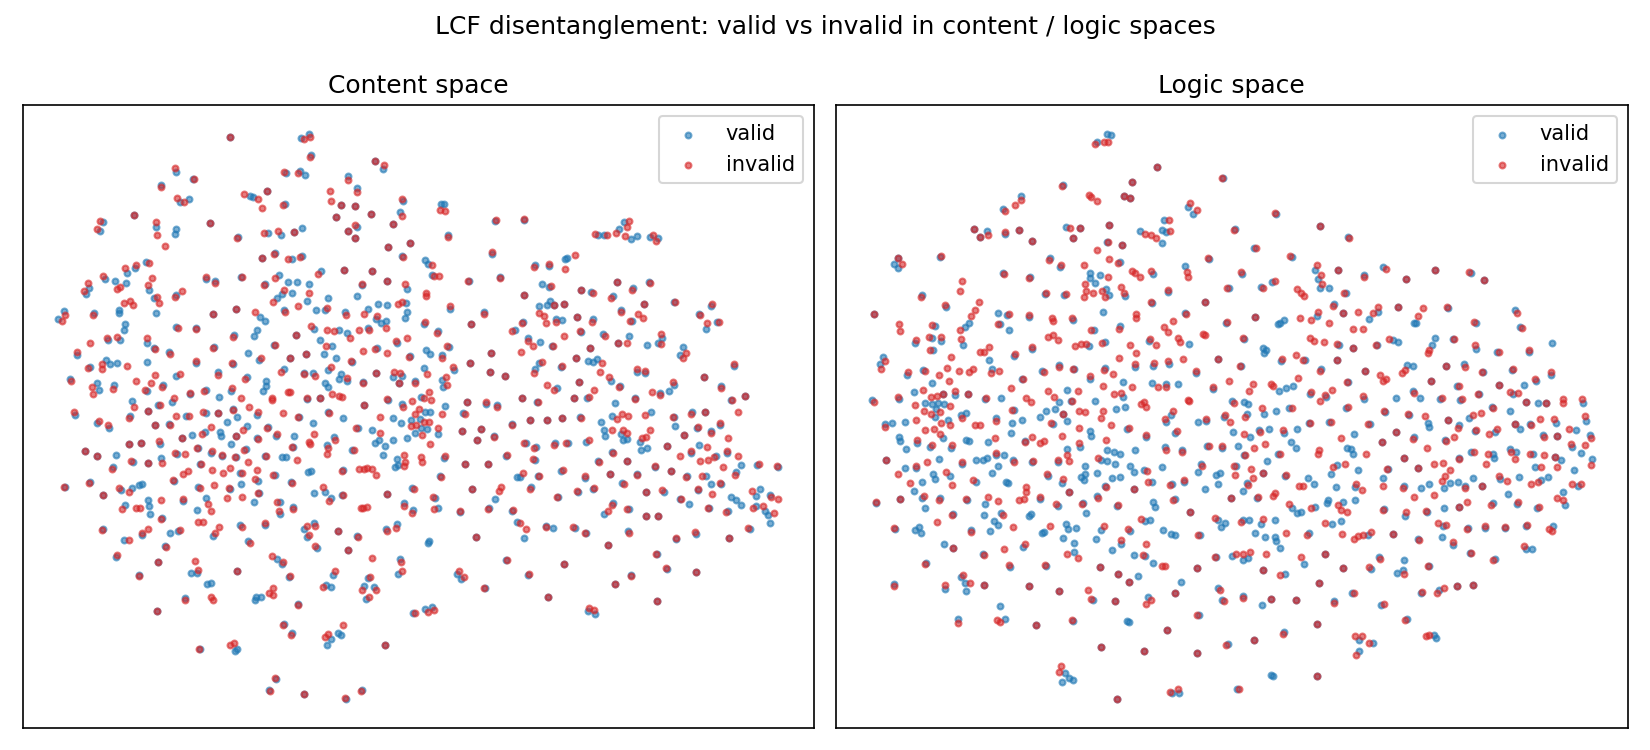
\includegraphics[width=\columnwidth]{figures/tsne_content_logic.png}
\caption{검증 표현의 t-SNE. 타당(파랑)/비타당(빨강)이 \emph{두 공간 모두}에서 혼재하며,
논문이 보고한 논리 공간 분리는 나타나지 않는다(분리도 $\approx\!0.66$).}
\label{fig:tsne}
\end{figure}

\paragraph{오류 식별.}
분리 방향이 없으므로 조정은 도움이 될 수 없다(표 \ref{tab:ident}). 논문 강도
$\eta{=}4.5$에서 정확도는 $69.6\!\to\!63.7$로 \emph{하락}한다. $\eta$ 스윕(표
\ref{tab:eta})도 같은 양상을 확인한다. $\eta\!\le\!2$에서는 중립, 그 이상에서는 유해하다.
비정보적 방향으로의 큰 이동이 표현을 손상시킬 뿐이기 때문이다. (우리 베이스라인은 논문의
$49\%$보다 훨씬 높은데, 선택지 구성이 타당 보기를 고르기 쉽게 만들기 때문이다. 이는
\S\ref{sec:analysis}에서 논의하는 평가 프로토콜 차이이다.)

\begin{table}[t]
\centering\small
\begin{tabular}{lcc}
\toprule
오류 식별 (n=204) & 정확도 & $\Delta$Prob \\
\midrule
원본 (Vicuna) & 69.6 & $+0.344$ \\
\;+LCF ($\eta{=}4.5$) & 63.7 & $+0.300$ \\
\midrule
\textit{논문 (Vicuna)} & \textit{49.0$\to$71.6} & --- \\
\bottomrule
\end{tabular}
\caption{본 설정에서 LCF는 식별 정확도를 오히려 낮춘다.}
\label{tab:ident}
\end{table}

\begin{table}[t]
\centering\small
\begin{tabular}{lccccccc}
\toprule
$\eta$ & 원본 & 0.25 & 0.5 & 1.0 & 2.0 & 4.5 & 8.0 \\
\midrule
정확도 & 71.7 & 71.7 & 71.7 & 72.5 & 71.7 & 68.3 & 65.8 \\
\bottomrule
\end{tabular}
\caption{조정 강도 $\eta$에 따른 식별 정확도(n=120). 중립 후 유해해지며, 의미 있는
개선을 주는 $\eta$는 없다.}
\label{tab:eta}
\end{table}

\paragraph{결론 생성.}
생성은 공정한 검증이다. 베이스라인의 타당 결론 비율이 $36.2\%$(Claude-Sonnet-4.6 판별)에
불과해 개선 여지가 충분하다. 그러나 LCF는 그 여지를 취하지 못한다(표 \ref{tab:gen}).
모든 강도에서 타당성이 정체 혹은 하락하고, $\eta{=}4.5$에서는 퍼플렉시티가 급격히
나빠진다($1.49\!\to\!2.98$). 이는 큰 $\eta$가 유창성을 해친다는 논문 관찰과 일치한다.
출력을 직접 살펴보면 LCF는 표현을 바꾸지만 논문의 개선 출력이 보이는 헤징(``\textit{may}'',
``\textit{not necessarily}'')을 더하지 못하며, 때로는 새로운 오류를 만들어 낸다.

\begin{table}[t]
\centering\small
\begin{tabular}{lcccc}
\toprule
생성 (n=80) & 원본 & $\eta$0.5 & $\eta$2.0 & $\eta$4.5 \\
\midrule
Valid\% (Claude 판별) & \textbf{36.2} & 35.0 & 31.2 & 35.0 \\
Perplexity & 1.49 & 1.50 & 1.57 & 2.98 \\
\bottomrule
\end{tabular}
\caption{어떤 $\eta$에서도 생성 타당성은 개선되지 않으며, 큰 $\eta$는 유창성을 해친다.
(논문: Vicuna $58.8\!\to\!75.0$.)}
\label{tab:gen}
\end{table}

\paragraph{통제 실험.}\label{sec:controlled}
실패의 원인을 좁히기 위해 다른 모든 조건을 고정한 채 가장 유력한 두 교란 요인을
변화시켰다(표 \ref{tab:ctrl}). \emph{추론 정밀도}: 4-bit 대신 fp16으로 재추출해도 최대
분리도는 $0.66\!\to\!0.67$로 거의 변화가 없다. 양자화가 원인이 아니다. \emph{라벨 품질}:
모든 타당 결론을 Claude-Sonnet-4.6으로 재생성하면(Vicuna와 달리 ``not visiting Europe
\emph{may be} why\ldots''처럼 올바르게 헤징) 분리도가 오히려 $0.57$로 \emph{하락}한다.
최소 편집된 타당/비타당 쌍은 텍스트가 더 유사해 공유 토큰에서 분리가 더 어려워지기
때문이다. 어느 개입도 메커니즘을 복구하지 못한다.

\begin{table}[t]
\centering\small
\begin{tabular}{lc}
\toprule
설정 (검증셋 분리도) & 최대 탭 \\
\midrule
4-bit, Vicuna 라벨 (주 설정) & 0.66 \\
fp16, Vicuna 라벨 & 0.67 \\
4-bit, Claude 라벨 (고품질) & 0.57 \\
\textit{우연 수준} & \textit{0.50} \\
\bottomrule
\end{tabular}
\caption{통제 실험: fp16도 고품질 라벨도 논리 공간을 분리 가능하게 만들지 못한다.}
\label{tab:ctrl}
\end{table}

\section{분석}\label{sec:analysis}
\paragraph{왜 실패하는가.} LCF의 효과는 하나의 전제에 달려 있다. 즉 대조 사영기가 은닉
공간을 타당 추론 영역과 비타당 추론 영역으로 가를 수 있다는 것이다. 우리 설정에서는 이
영역 구조가 부재한다(그림 \ref{fig:tsne}; 분리도 $\approx$ 우연). 학습 신호는 \emph{동일
내용 최소 쌍}이다. 동일 토큰의 차이는 오직 주변 논리 문맥뿐이므로 그 토큰에서의 타당성
신호는 내용에 비해 미약하고, 통제 실험이 보여주듯 더 나은 정밀도나 더 깨끗한 라벨로도
증폭되지 않는다. 오히려 고품질 라벨은 비타당 텍스트와 단어 차이가 더 적어 \emph{해롭다}.
분리 방향이 없으니 전역 조정 벡터는 잡음에 가깝고, 이를 큰 $\eta$로 10개 층에 적용하면
두 과제 모두 예측대로 악화된다.

\paragraph{재현된 것과 되지 않은 것.} LCF \emph{모듈}은 건전하다. 진짜 논리 축이 있는
합성 데이터에서는 주장대로 분리·구분·조정한다. 재현되지 않은 것은 그러한 축이 LFUD 최소
쌍으로부터 7B 모델 은닉 표현에 존재하고 복원 가능하다는 경험적 \emph{전제}이다. 우리가
통제하지 못해 기여했을 차이로는 베이스 모델(Vicuna 대 논문의 6종), 다수의 미명시
하이퍼파라미터(대조 온도, 전역 대 층별 조정, 식별 선택지 구성), 그리고 발산하던 학습
절차가 있다. 우리 식별 베이스라인 또한 쉬운 선택지 구성으로 부풀려져 개선 여지가 적었는데,
이는 논문의 평가 프로토콜이 불완전하게 명시되었음을 상기시킨다.

\paragraph{방법의 강점과 한계.} 설계상 LCF는 매력적이다. 동결 백본에 붙는 작은
모듈($\sim$136\,MB)로 가역적·양방향적이며 해석 가능한 표적(논리 부분공간)을 가진다. 본
연구가 드러낸 한계는 표현 기하에 관한 강하고 모델/데이터 의존적일 수 있는 가정이다. 우리
결과는 적어도 더 작은 모델, 공격적 양자화, 자동 생성 학습 쌍의 조건에서 그 가정이
취약함을 시사한다.

\section{결론}
우리는 LCF를 충실히 재구현하고 합성 데이터로 핵심을 검증한 뒤 \textsc{Vicuna-7b}에서
통제된 재현을 수행하였다. 방법의 핵심 메커니즘인 분리 가능한 논리 부분공간이 발현되지
않았고, 그 결과 LCF는 두 과제 모두에서 논문의 개선을 재현하지 못했다. 통제 실험은
양자화와 라벨 품질을 원인에서 배제한다. 우리는 이를 부정적이지만 유용한 결과로 읽는다.
LCF의 재현에는 원 연구의 조건(전정밀도의 더 큰 모델, 정교하게 큐레이션된 학습 쌍, 그리고
미명시된 평가 세부)이 필요할 가능성이 높으며, 분리 가능성 가정 자체가 향후 연구에서 직접
검증될 가치가 있다.

\section*{Limitations}
본 재현은 자원 제약상 단일 베이스 모델(Vicuna-7b)과 4-bit 양자화를 사용하며, 6개 모델
전체를 다루지 않는다. 타당 결론은 자동 생성되었고(논문의 수작업 검수 부재), 타당성
판별기는 LLM 판별기로 GPT-4 판별기 및 별도 학습된 Llama-2 판별기를 대체한다. 식별 과제의
선택지 구성과 일부 하이퍼파라미터는 원 논문에 명시되지 않아 합리적 선택으로 채웠으며,
이로 인해 절대 수치는 논문과 직접 비교되지 않을 수 있다. 따라서 본 보고서의 부정적 결과는
``이 방법이 항상 작동하지 않는다''가 아니라 ``이러한 제약 조건에서는 재현되지 않는다''로
한정해 해석되어야 한다.

\section*{Acknowledgments}
본 재현은 공개 데이터셋 LFUD와 오픈소스 모델 Vicuna-7b를 사용하였으며, 타당 결론 생성 및
타당성 판별에 Anthropic Claude API를 활용하였다.

\bibliography{references}
\bibliographystyle{acl_natbib}

\appendix

\section{구현·재현 세부}
\label{sec:appendix}
전체 코드, 데이터 분할, 합성 단위 테스트(\texttt{tests/test\_lcf\_local.py}), 조정 강도
스윕, 통제 실험이 보고서에 동봉되어 있으며, \texttt{run\_real.sh}는 깨끗한 체크아웃에서 모든
수치를 재현한다. LCF 모듈은 2층 MLP 사영기(출력 1024차원)와 단일 헤드 교차 어텐션 디코더로
구성되며, 어텐션·MLP 출력 뒤 순방향 훅(forward hook)으로 부착된다. 학습 데이터는 535개
항목에서 Vicuna 기준 9{,}336쌍, Claude 라벨 기준 12{,}048쌍을 추출하였다.

\end{document}
